\documentclass[
    10pt,
    aspectratio=169,
    xcolor={dvipsnames},
    spanish,
    % handout,
    % notes=only,
    % notes,
    ]{beamer}

% BEAMER SETTINGS
\setbeamerfont{section in toc}{size=\normalsize, shape=\bfseries}
\mode<presentation>{
    \usetheme{Antibes}
    \setbeamercovered{transparent}
    \usecolortheme{rose}
    \setbeamertemplate{navigation symbols}{}
    }
\useoutertheme{infolines}
% PACKAGES
% \usepackage[spanish]{babel}  % uncomment for Spanish support
\usepackage{tikz,pgfplots}
\pgfplotsset{compat=1.13}
\usetikzlibrary{calc}
\usepackage{subcaption}
\usepackage{graphicx}
\graphicspath{{figures}}
\usepackage{booktabs}
\usepackage{upgreek}
\usepackage{commath}
\usepackage{amsmath,amsthm,amssymb,mathtools,mathrsfs}
\usepackage{cancel}
\usepackage{fontawesome5}
\usepackage{enumerate}
\usepackage{tensor}
\usepackage[font=footnotesize]{caption}
\usepackage{wasysym}

\usepackage[skins,theorems]{tcolorbox}
\tcbset{
    highlight math style={
        enhanced,
        coltext=black,
        colframe=black,
        colback=lightgray,
        arc=0pt,
        boxrule=.5pt
        }
}

% REFERENCES AND OTHERS
\usepackage{aas_macros}
\usepackage{natbib}
\bibpunct{(}{)}{;}{a}{}{,}

\usepackage{siunitx}
\sisetup{
    range-phrase=\text{--},
    range-units=single,
    separate-uncertainty=true,
    print-unity-mantissa=false
    }
\DeclareSIUnit{\gauss}{G}
\DeclareSIUnit{\jansky}{Jy}
\renewcommand{\figurename}{Fig.}

\usepackage{hyperref}
\hypersetup{
    % bookmarks=true,
    unicode=true,
    pdftoolbar=true,
    pdfmenubar=true,
    pdffitwindow=false,
    pdfstartview={FitH},
    pdftitle={ISI-Free Linear Combination Pulses with Better Performanc},
    pdfauthor={Erik Saez A.},
    pdfcreator={Erik Saez A.},
    pdfnewwindow=true,
    colorlinks=true,
    linkcolor=RoyalBlue,
    citecolor=RoyalBlue,
    urlcolor=RoyalBlue
    }

\title[Auxiliar \#4 - Circuitos Electricos Analogicos]{\bfseries Auxiliar \#4 - Circuitos Electricos Analogicos}
\subtitle{Diodos}
\author[Erik Saez A.]{Erik Saez A.}
\institute[UChile]{Department of Electrical Engineering \\ Universidad de Chile}

\date{\today}

\begin{document}

\begin{frame}
  \titlepage
  \centering
  \faIcon{envelope} \href{mailto:erik.saez@ug.uchile.cl}{erik.saez@ug.uchile.cl} \hspace{.2cm}
  \faIcon{github} \href{https://github.com/ErikSaezA}{GitHub} \hspace{.2cm}
  \faIcon{discord} \href{https://discord.gg/ubthV3cudQ}{Discord}
\end{frame}
\begin{frame}
  \frametitle{Contenidos}
  \centering
  \begin{columns}
    \begin{column}{0.4\textwidth}
      \tableofcontents
    \end{column}
    \begin{column}{0.5\textwidth}
      \begin{figure}
        \centering
        
\includegraphics[width=\textwidth]{fcfm_die}
        \caption{Facultad de Ciencias Físicas y Matemáticas, Universidad de Chile.}
      \end{figure}
    \end{column}
  \end{columns}  
\end{frame}
%%%%%%%%%%%%%%%%%%%%%%%%%%%%%%%%%%%%%%%%%%

\section{Resumen de Conceptos}



%%%%%%%%%%%%%%%%%%%%%%%%
\section{Pregunta 1}
\begin{frame}{Pregunta \#1}
  \footnotesize
  \begin{block}{Enunciado Pregunta \#1}
    Para el circuito de la Figura~\ref{fig:1}, si utiliza la expresión exacta $I(v_D)$ del diodo, plantee la ecuación que se debe satisfacer. Plantee un modelo de aproximación para el diodo que permita resolver los voltajes y corrientes en el circuito. Sea explícito en los modelos y supuestos utilizados.
\begin{equation}
  i_D = I_s \left( e^{v_D/(\eta V_T)} - 1 \right)
\end{equation}
\end{block}
\begin{figure}[H]
    \centering
    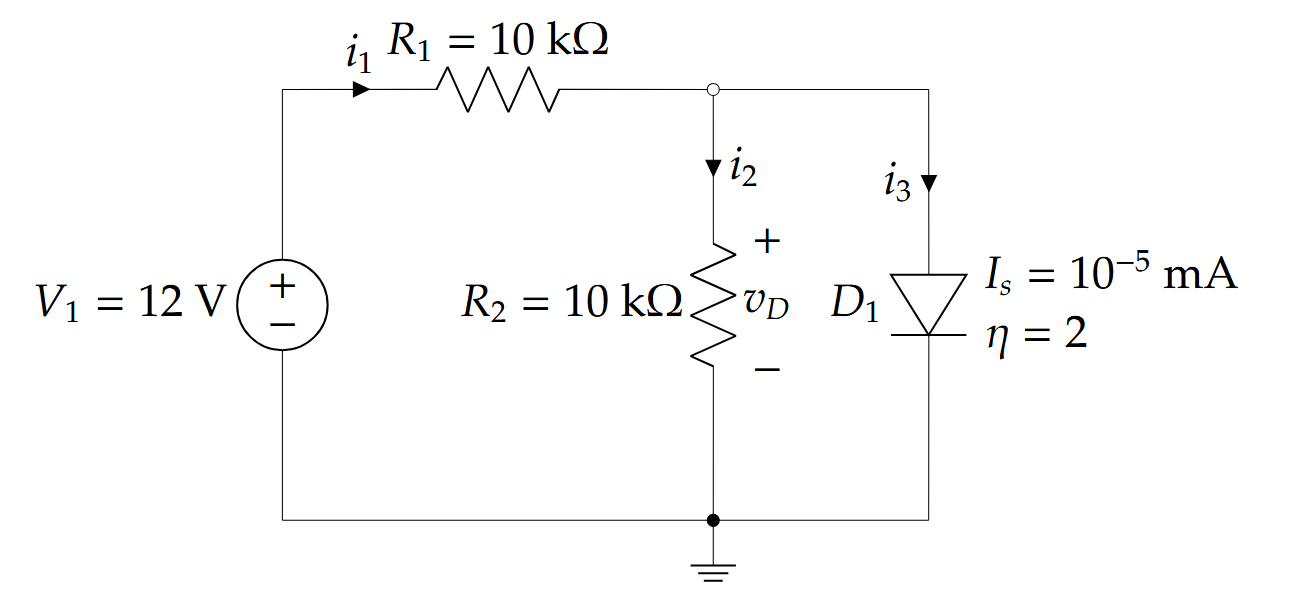
\includegraphics[width=0.55\textwidth]{Auxiliar_4_1}
  \caption{Circuito con Diodo.}
    \label{fig:1}
\end{figure}
\end{frame}
%------------------------
\begin{frame}{Pregunta \#1}
  \begin{figure}[H]
    \centering
    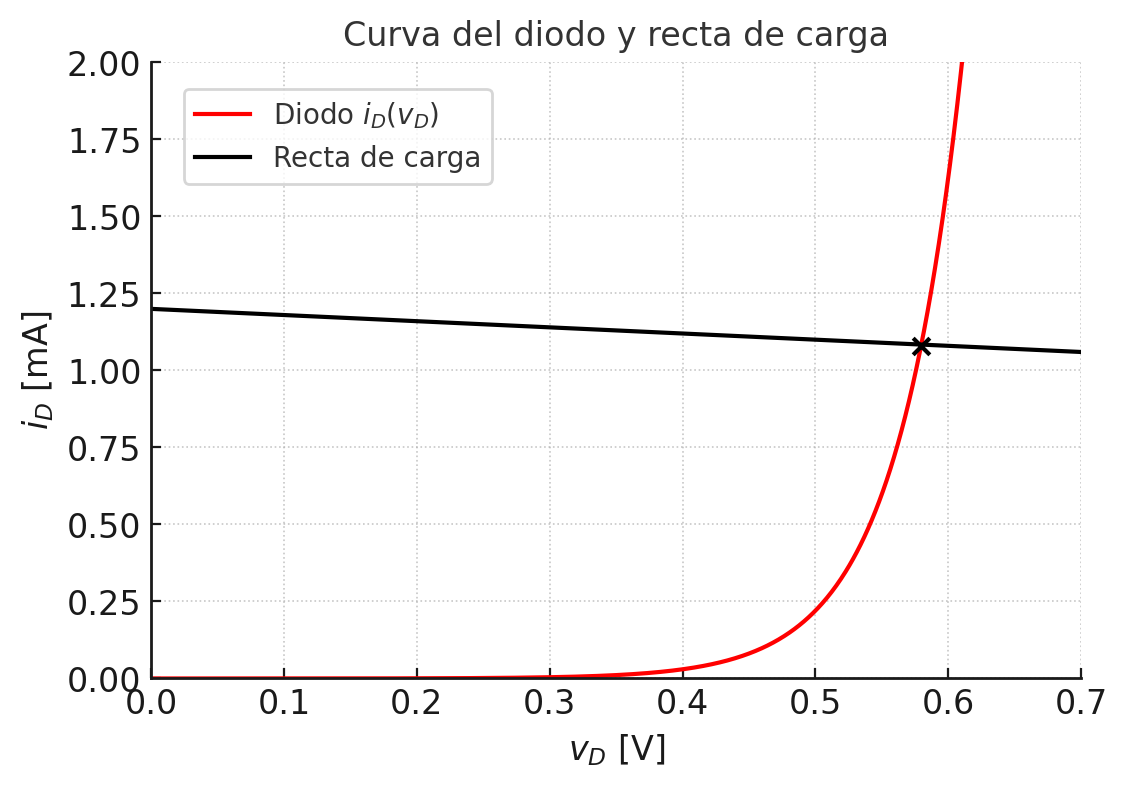
\includegraphics[width=0.55\textwidth]{Auxiliar_4_2}
    \caption{Curva característica del diodo y recta de carga. El punto de intersección indica la solución del circuito.}
    \label{fig:2}
\end{figure}
\end{frame}
%%%%%%%%%%%%%%%%%%%%%%
\section{Pregunta 2}
\begin{frame}{Pregunta \#2}
  \footnotesize
  \begin{block}{Enunciado Pregunta \#2}
 Un diodo Zener con característica $v$--$i$, como la mostrada en la Figura 5a), tiene un voltaje de Zener $V_{ZK}=3\ \mathrm{V}$. Determine la corriente $i_X$ en los dos circuitos mostrados en la figura \ref{fig:ex4c}. Sea explícito en los modelos y supuestos utilizados.  
  \end{block}

  \begin{figure}[H]
  \centering

  \begin{subfigure}[b]{0.48\textwidth}
    \centering
    % ajusta a \linewidth para ocupar bien cada subfigura
    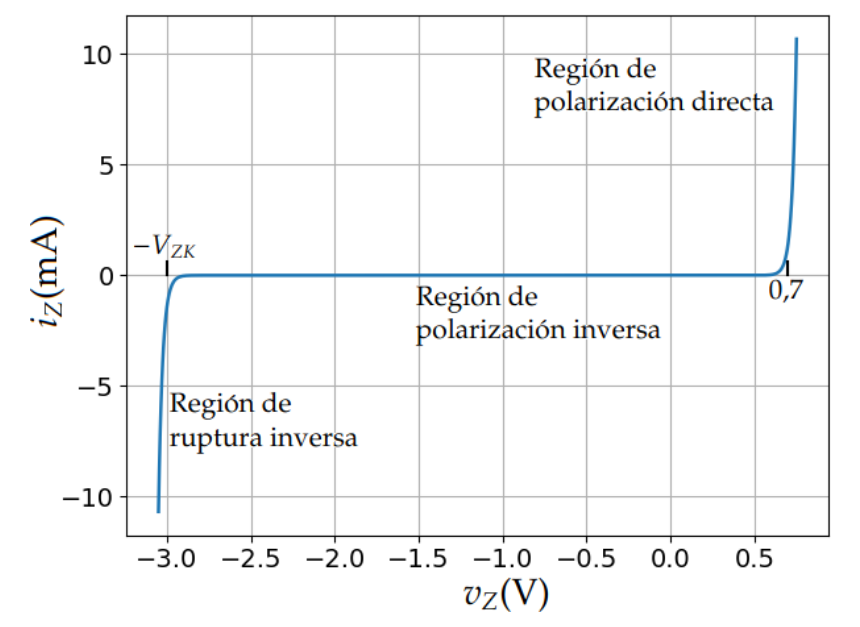
\includegraphics[width=0.9\linewidth]{Auxiliar_4_5}
    \caption{Caso (a): equivalente de Thévenin con el diodo Zener en la orientación mostrada; se marca $v_X$ y la polaridad adoptada para $v_Z$.}
    \label{fig:ex4a}
  \end{subfigure}\hfill
  \begin{subfigure}[b]{0.48\textwidth}
    \centering
    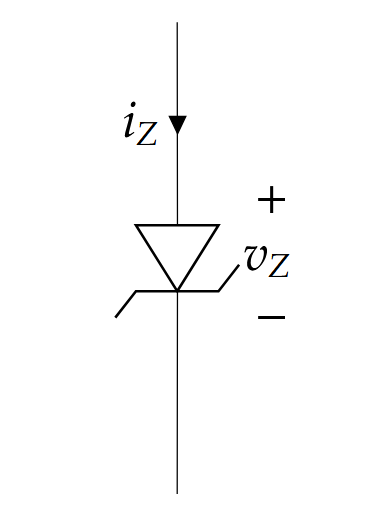
\includegraphics[width=0.45\linewidth]{Auxiliar_4_6}
    \caption{Caso (b): mismo equivalente con la orientación del diodo invertida respecto a (a); compare la polaridad y la dirección de $i_X$.}
    \label{fig:ex4b}
  \end{subfigure}

  \caption{Comparación de los dos casos propuestos: (a) y (b). Las polaridades indicadas definen la referencia de $v_Z$ y la dirección positiva de la corriente $i_X$.}
  \label{fig:ex4ab}
\end{figure}
\end{frame}

\begin{frame}{Pregunta \#2}
  \begin{figure}[H]
    \centering
    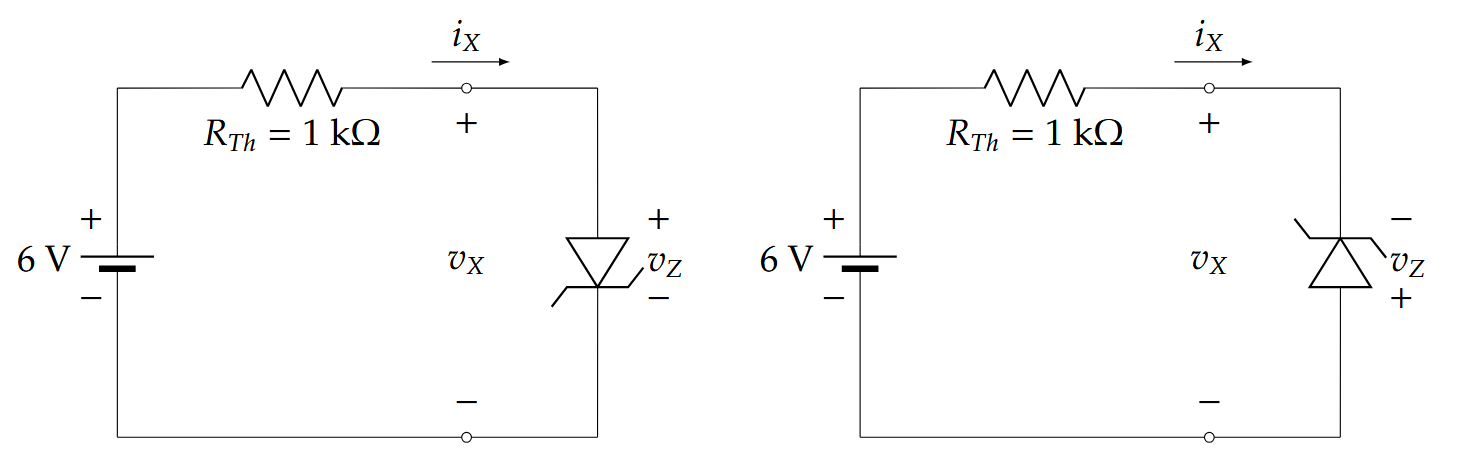
\includegraphics[width=0.8\textwidth]{Auxiliar_4_7}
      \caption{Característica $v$--$i$ del diodo Zener, mostrando las regiones de polarización directa, inversa y de ruptura inversa, así como los valores típicos de voltaje y corriente.}
    \label{fig:ex4c}
  \end{figure}
\end{frame}
%%%%%%%%%%%%%%%%%%%%%%%%
\begin{frame}{Pregunta \#2}
  \begin{figure}[H]
  \centering
  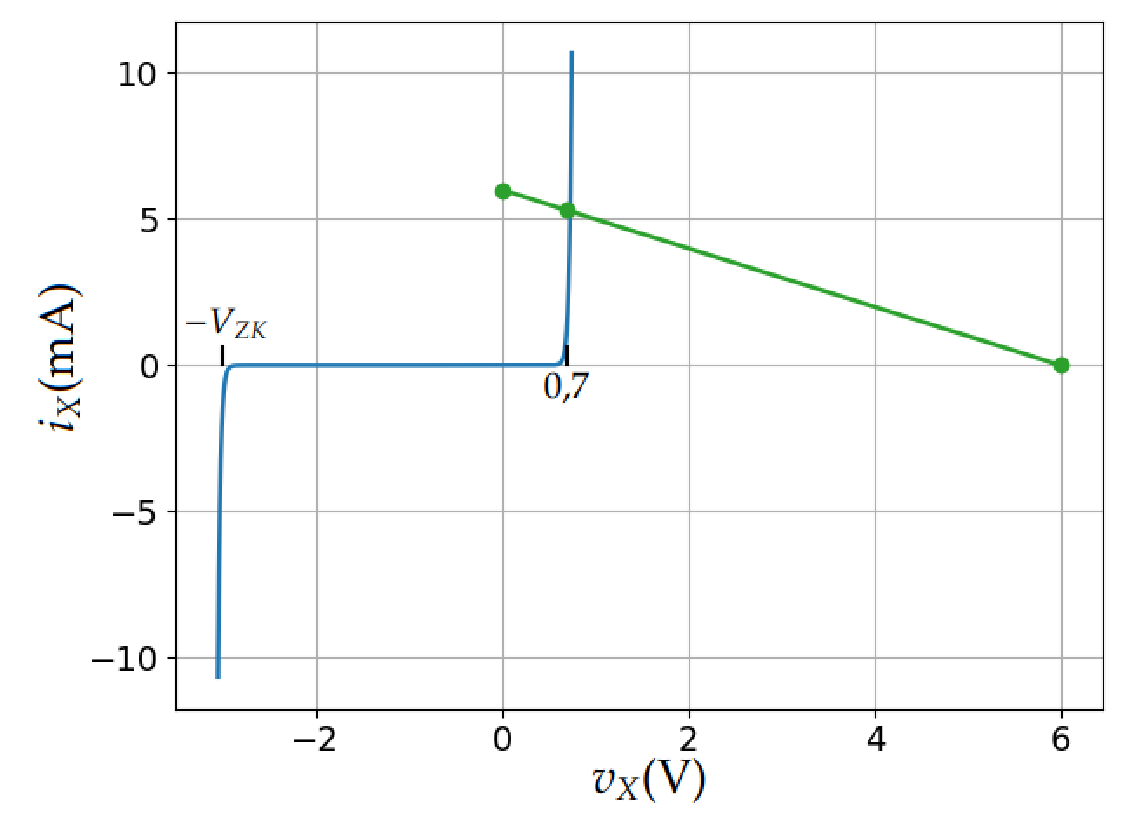
\includegraphics[width=0.5\textwidth]{Auxiliar_4_8}
  \caption{Curva característica \(v\)-\(i\) del voltaje \(v_X\) (curva azul). 
  Se intersecta la recta de carga (curva verde) con esta curva exponencial, para encontrar el punto de operación. 
  Los puntos verdes de los extremos de la recta corresponden a los puntos usados para generarla. 
  El punto verde del medio es el punto de operación del diodo si asumimos que el voltaje máximo es de \(0{,}7~\text{V}\). 
  Notemos que este punto está suficientemente cerca de la intersección real entre ambas curvas, por lo que el modelo de fuente de voltaje es una aproximación razonable.}
  \label{fig:carac-v-i}
\end{figure}
\end{frame}
%%%%%%%%%%%%%%%%%%%%%%%%
\begin{frame}{Pregunta \#2}
\begin{figure}[H]
  \centering
  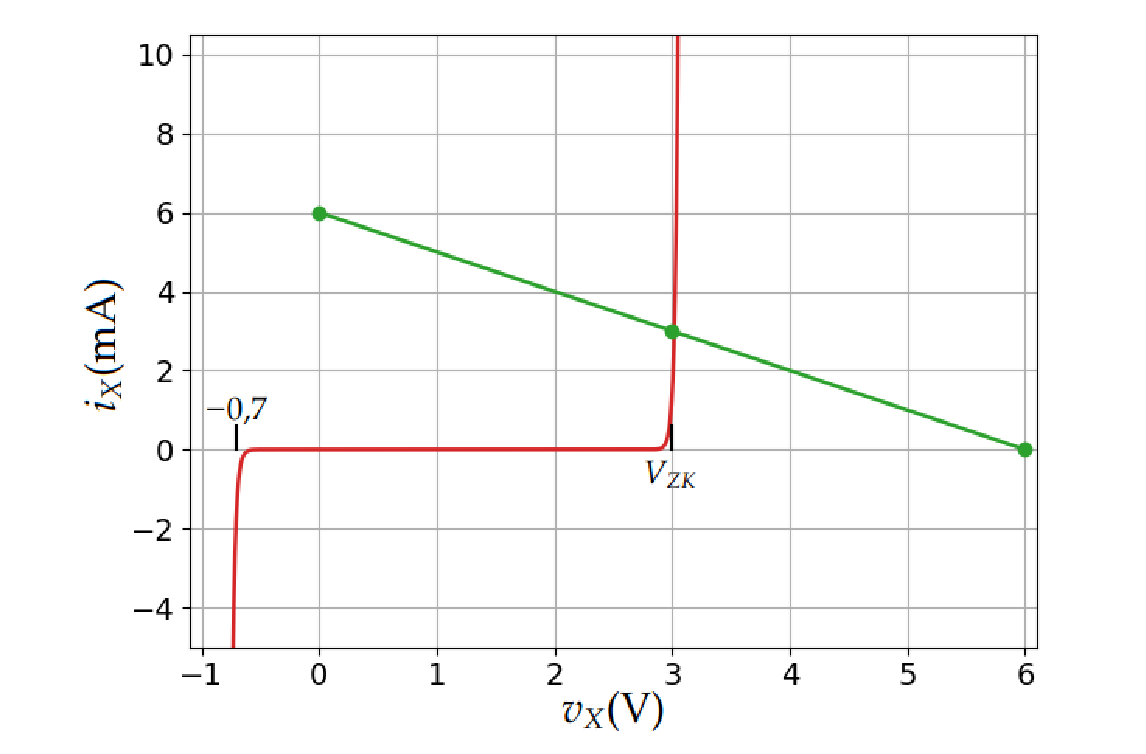
\includegraphics[width=0.5\textwidth]{Auxiliar_4_9}
  \caption{Característica $v$--$i$ del voltaje $v_X$ (recordar que el diodo Zener está invertido, por lo que la región de polarización inversa, que corresponde a voltajes negativos para el diodo Zener, en este gráfico está como voltajes positivos. Notar que la corriente también cambia de signo por la misma razón). Se intersecta la recta de carga con esta curva exponencial, para encontrar el punto de operación.}
  \label{fig:iv-diodo}
\end{figure}
\end{frame}
%%%%%%%%%%%%%%%%%%%%%%%%
\begin{frame}{Pregunta \#3}
  \footnotesize
  \begin{block}{Enunciado Pregunta \#3}
  Para el circuito de la figura 6, bosqueje el voltaje en el diodo y la corriente en el diodo como función del tiempo. Sea explícito en los valores de las gráficas, así como en los modelos y supuestos utilizados.
  \end{block}
\begin{figure}[H]
  \centering
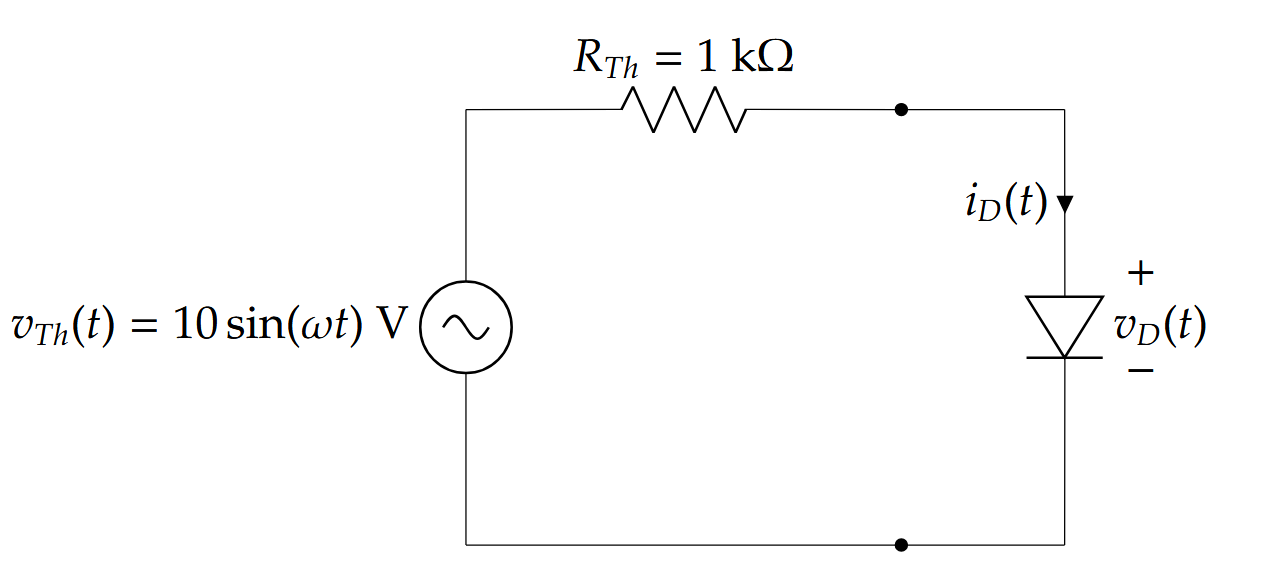
\includegraphics[width=0.65\textwidth]{Auxiliar_4_12}
  \caption{Circuito con diodo y fuente de voltaje senoidal.}
  \label{fig:3}
\end{figure}
\end{frame}
%%%%%%%%%%%%%%%%%%%%%%%%%
\begin{frame}{Pregunta \#3}
\begin{table}[H]
  \centering
  \begin{tabular}{c c c c c c}
    \hline
    Punto de operación & $\omega t$ & $\sin(\omega t)$ & $v_{Th}(t)$ (V) & $v_D$ (V) & $i_D$ (mA) \\
    \hline
    3 & 0 & 0 & 0 & 0 & 0 \\
    2 & $\pi/6$ & 1/2 & 5 & 0.7 & 4.3 \\
    1 & $\pi/2$ & 1 & 10 & 0.7 & 9.3 \\
    2 & $5\pi/6$ & 1/2 & 5 & 0.7 & 4.3 \\
    3 & $\pi$ & 0 & 0 & 0 & 0 \\
    4 & $7\pi/6$ & -1/2 & -5 & -5 & $\approx -I_s$ \\
    5 & $3\pi/2$ & -1 & -10 & -10 & $\approx -I_s$ \\
    4 & $11\pi/6$ & -1/2 & -5 & -5 & $\approx -I_s$ \\
    3 & $2\pi$ & 0 & 0 & 0 & 0 \\
    \hline
  \end{tabular}
  \caption{Valores de voltaje y corriente en el diodo para distintos puntos de operación durante un ciclo senoidal.}
  \label{tab:diodo-operacion}
\end{table}
\end{frame}
%------------------------
\begin{frame}{Pregunta \#3}
\begin{figure}[H]
    \centering
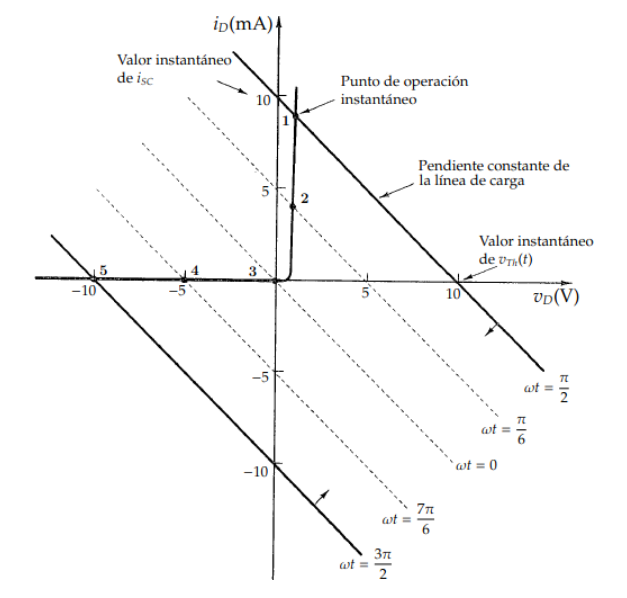
\includegraphics[width=0.5\textwidth]{Auxiliar_4_17}
    \caption{Voltaje de Thévenin $v_{Th}(t)$ como función del tiempo.}
    \label{fig:voltaje-th}
\end{figure}
  \end{frame}
%------------------------
\begin{frame}{Pregunta \#3}

\begin{figure}[H]
  \centering
  \begin{subfigure}[b]{0.48\textwidth}
    \centering
    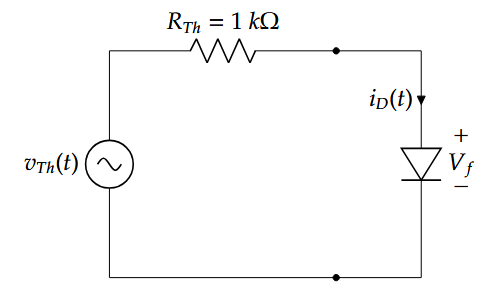
\includegraphics[width=0.9\linewidth]{Auxiliar_4_13}
    \caption{Circuito equivalente cuando el diodo no conduce ($i_D(t) = 0$).}
    \label{fig:diodo-abierto}
  \end{subfigure}\hfill
  \begin{subfigure}[b]{0.48\textwidth}
    \centering
    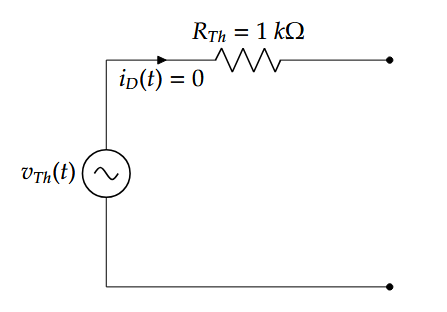
\includegraphics[width=0.9\linewidth]{Auxiliar_4_14}
    \caption{Circuito equivalente cuando el diodo conduce ($i_D(t) > 0$).}
    \label{fig:diodo-conduce}
  \end{subfigure}
  \caption{Modelos de operación del circuito con diodo: (a) abierto, (b) conduciendo.}
  \label{fig:diodo-operacion-casos}
\end{figure}
\end{frame}

%------------------------
\begin{frame}{Pregunta \#3}
\begin{figure}[H]
    \centering
    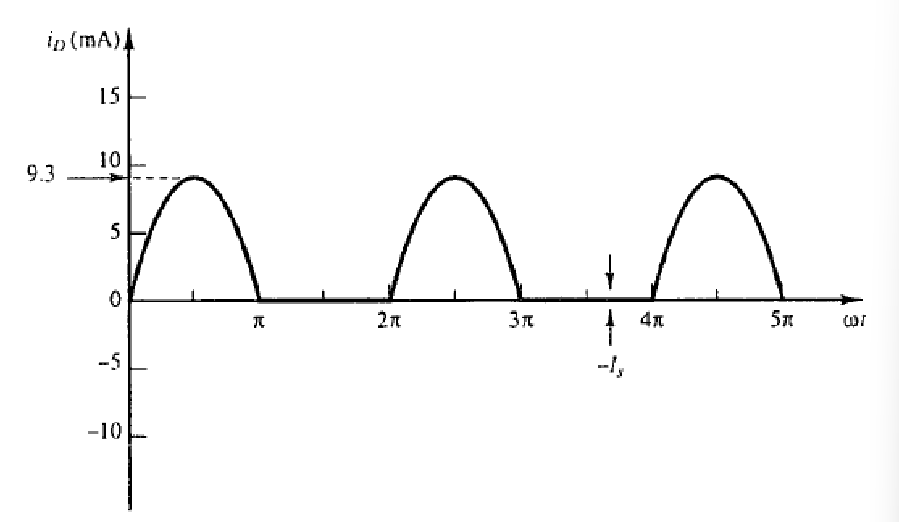
\includegraphics[width=0.55\textwidth]{Auxiliar_4_16}
  \caption{Sólo pasa corriente por el diodo cuando el voltaje es positivo (polarización directa en el diodo), porque cuando es negativo (polarización inversa en este diodo), el diodo actúa como un circuito abierto.}
    \label{fig:voltaje-corriente-diodo-detalle}
\end{figure}
\end{frame}
%------------------------
\begin{frame}{Pregunta \#4}
  \begin{block}{Enunciado Pregunta \#4}
   Sea el esquema visto en la Figura~\ref{fig:P2_17}, responda lo siguiente, considerando la fuente de voltaje que ahí aparece.
\begin{enumerate}
    \item Represente (bosqueje) $v_o$ en función del tiempo para el circuito de la Figura~\ref{fig:P2_17} (lado izquierdo) con la entrada mostrada. Suponga $V_\gamma = 0$.
    \item Represente (bosqueje) $v_o$ en función del tiempo para el circuito de la Figura~\ref{fig:P2_17} (lado derecho). La entrada es senoidal y está dada por $v_i(t) = 10 \sin(\omega t)\,\text{V}$. Suponga $V_\gamma = 0$.
\end{enumerate}
  \end{block}
\begin{figure}[H]
    \centering
    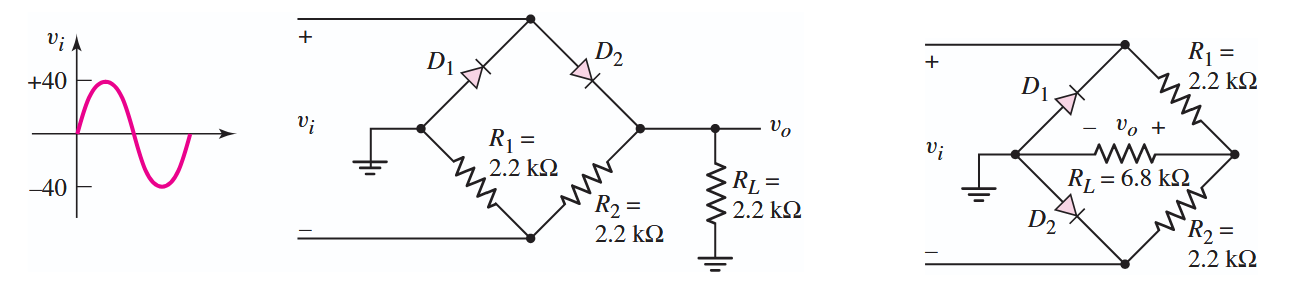
\includegraphics[width=0.7\textwidth]{Auxiliar_4_18}
  \caption{Esquema del circuito con diodos.}
    \label{fig:P2_17}
\end{figure}
\end{frame}
%------------------------
\begin{frame}{Pregunta \#4}
  \begin{figure}[H]
    \centering
    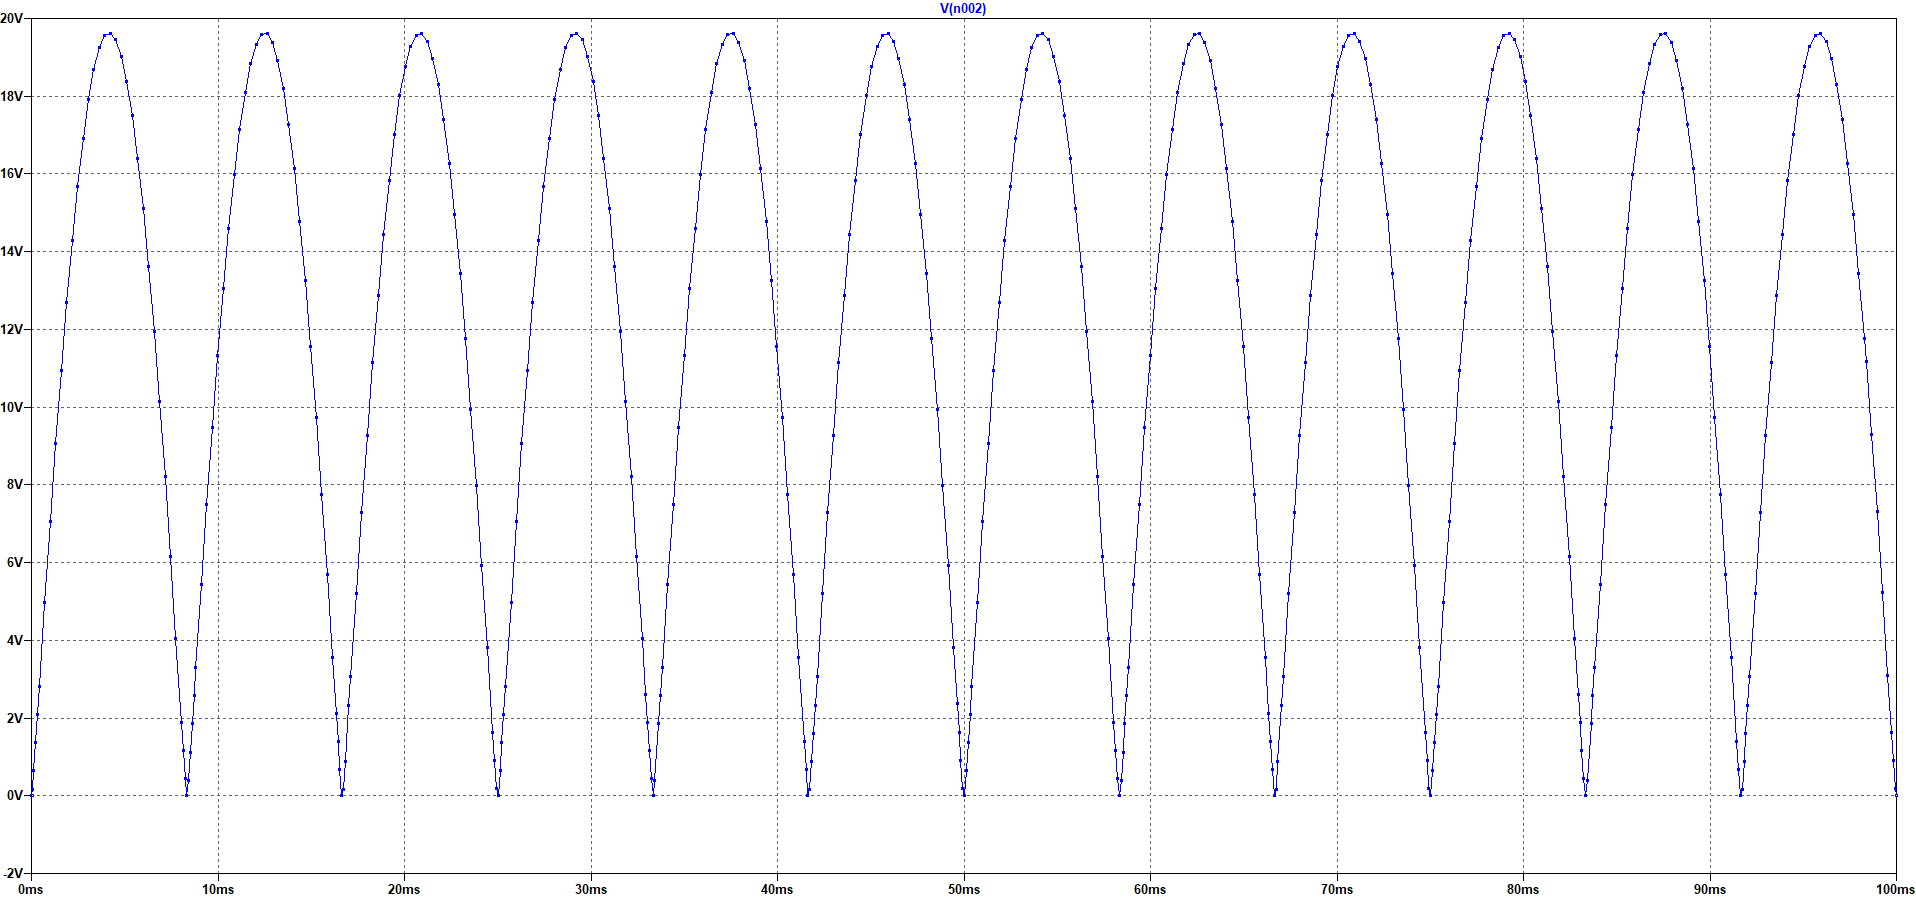
\includegraphics[width=0.7\textwidth]{Auxiliar_4_21}
  \caption{Sólo pasa corriente por el diodo cuando el voltaje es positivo (polarización directa en el diodo), porque cuando es negativo (polarización inversa en este diodo), el diodo actúa como un circuito abierto.}
    \label{fig:voltaje-corriente-diodo-detalle}

\end{figure}
\end{frame}
%%%%%%%%%%%%%%%%%%%%%%%%%
\end{document}
